\section{Provide an in-depth analysis of your primary research topic for this course
(as selected in Assignment 3). In particular, you should provide the following elements. For each of these elements, provide a table that summarizes your findings.}

\subsection{A summary and categorization of the information visualization techniques employed.}
Upon examining the research literature, four primary attributes of the data to be visualized can be identified: How similar different result items are to one another, what their relationship is, how relevant a specific result item is in respect to the search terms, what language the document is in, and how big items are in document size. The most commonly used techniques for encoding these attributes are based on position, connection, color, and size. For position, Self-organized Maps, putting items into distinct, unrelated areas, and plotting them in a multidimensional space - or grid - such as a coordinate system are used. Connection is always visualized by providing connecting lines. For color, items can be either colored using distinct color entities or a monotonous spectrum. The size can be either used by scaling the entire icon representing a result item, or by using the item's different dimensions. \\
Table \ref{tab:techniques:encoding} displays the utilized encoding techniques in research literature.
	
\begin{center}
\begin{longtable}{ll|lllll}
			
			&				
			& \textbf{Similarity}	
			& \textbf{Relationship}	
			& \textbf{Relevance}	
			& \textbf{Language} 
			& \textbf{Size}
  \\ \hline
				\textbf{Position}
			&	\footnotesize{Self-organized Maps}
			& \cite{Benjamin2008, Roussinov1999}
	\\
			
			& \footnotesize{Distinct Areas}
			& \cite{Einsfeld2006, Mukherjea1999, Rauber2000, Tvarozek2008}
	\\
			
			& \footnotesize{Multidimensional Grid}
			& \cite{Mukherjea1996, Paulovich2008, Sebrechts1999, Weippl2001}
			& \cite{Nowell1996}
			& \cite{Einsfeld2006, Konchady1998, Nowell1996}*
	\\
				\textbf{Connection}
			& \footnotesize{Connecting Lines}
			&
			& \cite{Einsfeld2006, Mukherjea1999, Paulovich2008, Zaina2005}
	\\
				\textbf{Color}
			& \footnotesize{Distinct Color Entities}
			& \cite{Einsfeld2006}
			&
			& \cite{Mukherjea1999, Nowell1996}
			& \cite{Rauber2000}
	\\
			
			& \footnotesize{Color Spectrum}
			&
			&
			& \cite{Paulovich2008, Weiss2001}
	\\
				\textbf{Size}
			& \footnotesize{Scale}
			&
			&
			& \cite{Paulovich2008}
			&
			& \cite{Zaina2005}
	\\
	
			& \footnotesize{Dimensions}
			&
			&
			& \cite{Mukherjea1996}
			&
			& \cite{Rauber2000}
	\\
	\caption{Encoding techniques}
	\label{tab:techniques:encoding}
\end{longtable}
\end{center}
It should be noted, that ordinary search engines format their outcome as a one dimensional list ordered by relevance. This corresponds to position (*) in Table \ref{tab:techniques:encoding}. Obviously, most literature concentrates on visualizing similarities and relevance of result items with position and color based techniques being the ones most commonly used.

\subsection{A summary and categorization of the interaction techniques employed.}

There are three different primary methods for allowing the user to interactively manipulate a visualization: Displaying additional details on demand, allowing the user to refine the data set that is to be displayed, and to enable him to customize the presentation. Most techniques presented in the research literature concentrates on the first, thus practically following Shneiderman's overview-zoom-detail paradigm from \cite{Shneiderman1996}. Figure \ref{img:techniques:interaction} displays the different techniques found in the literature.
\begin{figure}[htbp]
  \begin{center}
    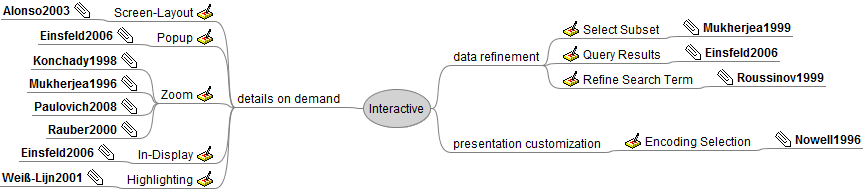
\includegraphics[width=6in]{exercises/img_technique_interaction.png}
    \caption{Interaction techniques}
    \label{img:techniques:interaction}
  \end{center}
\end{figure}

\subsection{A summary of the evaluation techniques employed.}
Three different primary domains can be identified that are evaluated by research literature: How well a visualization performs, how much it is accepted by users, and how easy it is for users to comprehend. Figure \ref{img:techniques:evaluation} displays the techniques discussed in literature.
\begin{figure}[htbp]
  \begin{center}
    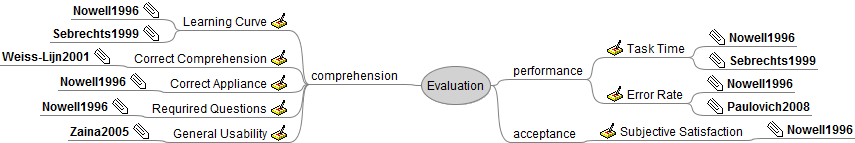
\includegraphics[width=6in]{exercises/img_technique_evaluation.png}
    \caption{Evaluation techniques}
    \label{img:techniques:evaluation}
  \end{center}
\end{figure}